\documentclass[a4paper,14pt,russian]{extreport} \usepackage{extsizes}
\usepackage{cmap} 
\usepackage[T2A]{fontenc}
\usepackage[utf8]{inputenc}
\usepackage[russian]{babel}
\usepackage{pscyr}
\usepackage{graphicx}  \usepackage{amssymb,amsfonts,amsmath,amsthm}  \usepackage{indentfirst} \usepackage[usenames,dvipsnames]{color}
\usepackage{makecell}
\usepackage{multirow}
\usepackage{ulem} 
\linespread{1.3} 
\renewcommand{\rmdefault}{ftm}
\frenchspacing
\usepackage{fancyhdr}
\pagestyle{fancy}
\fancyhf{}
\fancyhead[R]{\thepage}
\fancyheadoffset{0mm}
\fancyfootoffset{0mm}
\setlength{\headheight}{17pt} \renewcommand{\headrulewidth}{0pt} \renewcommand{\footrulewidth}{0pt} \fancypagestyle{plain}{\fancyhf{} \rhead{\thepage}}
\setcounter{page}{2} % начать нумерацию страниц с №2
\usepackage[tableposition=top]{caption}
\usepackage{subcaption}
\DeclareCaptionLabelFormat{gostfigure}{Рисунок #2} \DeclareCaptionLabelFormat{gosttable}{Таблица #2} \DeclareCaptionLabelSeparator{gost}{~---~}
\captionsetup{labelsep=gost} 
\captionsetup[figure]{labelformat=gostfigure}
\captionsetup[table]{labelformat=gosttable} \renewcommand{\thesubfigure}{\asbuk{subfigure}}
\usepackage{titlesec} 
\titleformat{\chapter}[display]
{\filcenter}
{\MakeUppercase{\chaptertitlename} \thechapter}     {8pt}    
{\bfseries}{} 
\titleformat{\section}
{\normalsize\bfseries}
{\thesection}{1em}{}
\titleformat{\subsection}     
{\normalsize\bfseries}
{\thesubsection}     
{1em}{}
\titlespacing*{\chapter}{0pt}{-30pt}{8pt} \titlespacing*{\section}{\parindent}{*4}{*4} \titlespacing*{\subsection}{\parindent}{*4}{*4}
\usepackage{geometry}
\geometry{left=3cm}
\geometry{right=1.5cm}
\geometry{top=2.4cm}
\geometry{bottom=2.4cm}
\usepackage{enumitem}
\makeatletter  
\AddEnumerateCounter{\asbuk}{\@asbuk}{м)} 
\makeatother
\setlist{nolistsep}
\renewcommand{\labelitemi}{-} \renewcommand{\labelenumi}{\asbuk{enumi})} \renewcommand{\labelenumii}{\arabic{enumii})}
\newcommand{\empline}{\mbox{} \newline}
\newcommand{\likechapterheading}[1]{
	\begin{center}
		\textbf{\MakeUppercase{#1}}
	\end{center}
	\empline}
\sloppy
\newcommand{\jj}{\righthyphenmin=20 \justifying}
\usepackage{tocloft}
\renewcommand{\cfttoctitlefont}{\hspace{0.38\textwidth} \bfseries\MakeUppercase}
\renewcommand{\cftbeforetoctitleskip}{-1em}
\renewcommand{\cftaftertoctitle}{\mbox{}\hfill \\ 
	\mbox{}\hfill{\footnotesize Стр.}\vspace{-2.5em}} \renewcommand{\cftchapfont}{\normalsize\bfseries \MakeUppercase{\chaptername} } \renewcommand{\cftsecfont}{\hspace{31pt}} \renewcommand{\cftsubsecfont}{\hspace{11pt}} \renewcommand{\cftbeforechapskip}{1em} 
\renewcommand{\cftparskip}{-1mm} \renewcommand{\cftdotsep}{1} \setcounter{tocdepth}{2} % задать глубину оглавления — до subsection включительно
\makeatletter
\renewcommand{\@dotsep}{2}     \newcommand{\l@likechapter}[2]{{\bfseries\@dottedtocline{0}{0pt}{0pt}{#1}{#2}}} \makeatother\newcommand{\likechapter}[1]{       
	\likechapterheading{#1}    
	\addcontentsline{toc}{likechapter}{\MakeUppercase{#1}}}
\usepackage[title,titletoc]{appendix}
\titleformat{\paragraph}[display]
{\filcenter}
{\MakeUppercase{\chaptertitlename} \thechapter}     {8pt}
{\bfseries}{}
\titlespacing*{\paragraph}{0pt}{-30pt}{8pt}
\newcommand{\append}[1]{
	\clearpage
	\stepcounter{chapter}  
	\paragraph{\MakeUppercase{#1}}
	\empline \addcontentsline{toc}{likechapter}{\MakeUppercase{\chaptertitlename~\Asbuk{chapter}\;#1}}}
\begin{document}
	\chapter{Эксперимент}
	Для проверки математических рассчётов было организовано 2 эксперимента: управление по моментам и управление по силам.	
	\section{Управление по силам}
		\begin{figure}[h]
			\centering		 
			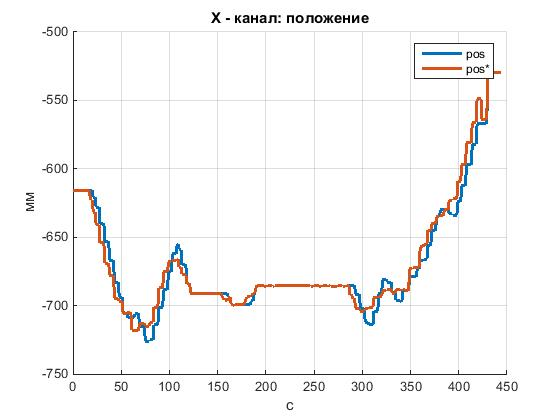
\includegraphics[width=5.5in]{./graph/posX.jpg}	
			\caption{
				\textbf{X - канал: положения}
			}     
			\label{fig_img41}
		\end{figure}
		\begin{figure}[h]
			\centering		 
			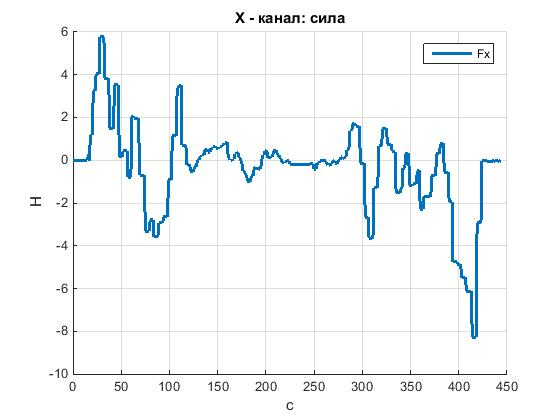
\includegraphics[width=5.5in]{./graph/powX.jpg}	
			\caption{
				\textbf{X - канал: силы}
				}
			\label{fig_img42}
		\end{figure}
		\begin{figure}[h]
			\centering		 
			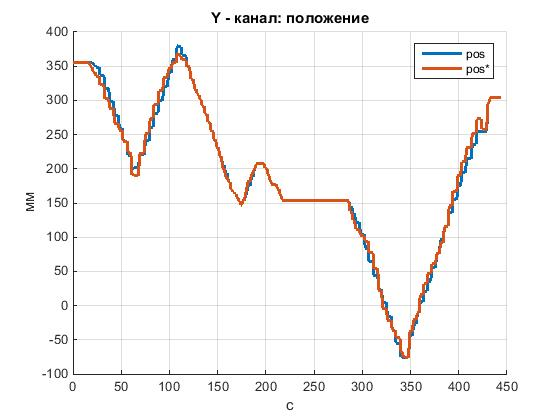
\includegraphics[width=5.5in]{./graph/posY.jpg}	
			\caption{
				\textbf{Y - канал: положения}
			}
			\label{fig_img43}
		\end{figure}
		\begin{figure}[h]
			\centering		 
			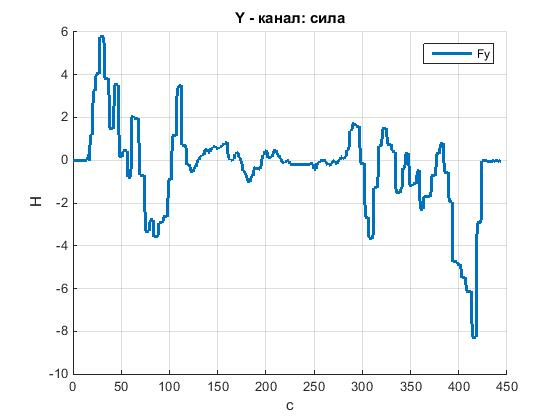
\includegraphics[width=5.5in]{./graph/powY.jpg}	
			\caption{
				\textbf{Y - канал: силы}
			}
			\label{fig_img44}
		\end{figure}
		\begin{figure}[h]
			\centering		 
			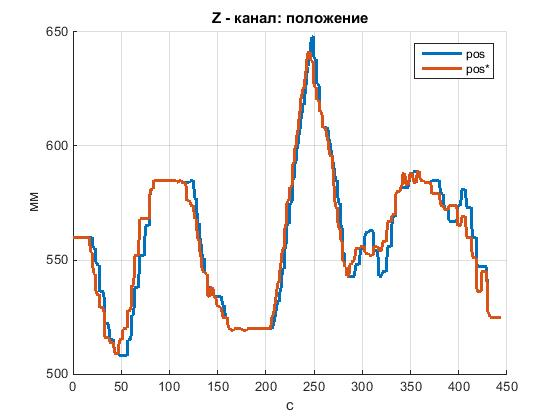
\includegraphics[width=5.5in]{./graph/posZ.jpg}	
			\caption{
				\textbf{Z - канал: положения}
			}
			\label{fig_img45}
		\end{figure}
		\begin{figure}[h]
			\centering		 
			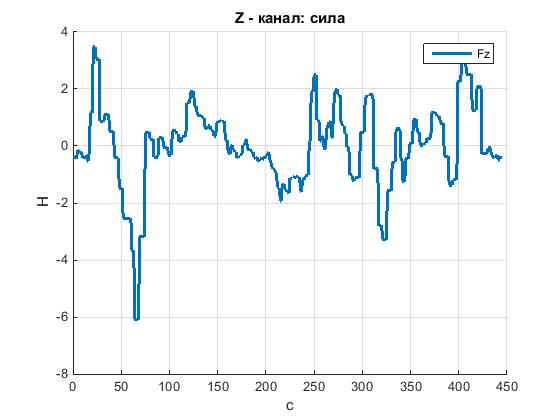
\includegraphics[width=5.5in]{./graph/powZ.jpg}	
			\caption{
				\textbf{Z - канал: силы}
			}
			\label{fig_img46}
		\end{figure}
	\section{Управление по моментам}
	\begin{figure}[h]
		\centering		 
		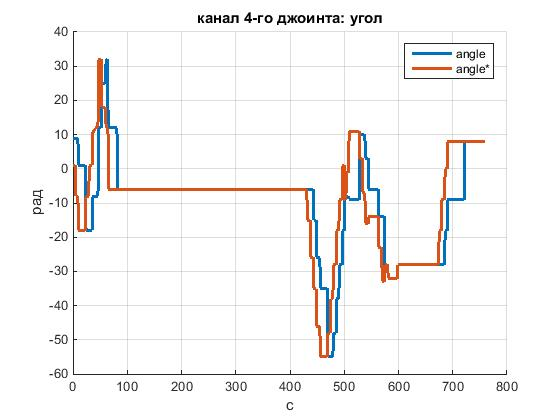
\includegraphics[width=5.5in]{./graph/j4.jpg}	
		\caption{
			\textbf{X - канал: положения}
		}     
		\label{fig_img51}
	\end{figure}
	\begin{figure}[h]
		\centering		 
		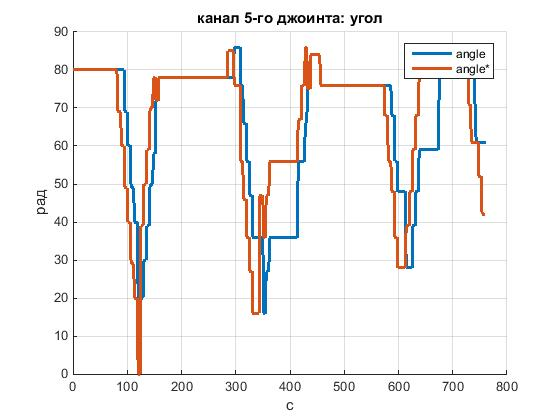
\includegraphics[width=5.5in]{./graph/j5.jpg}	
		\caption{
			\textbf{X - канал: силы}
		}
		\label{fig_img52}
	\end{figure}
	\begin{figure}[h]
		\centering		 
		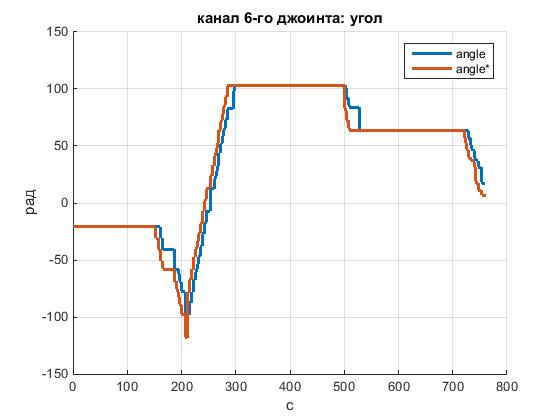
\includegraphics[width=5.5in]{./graph/j6.jpg}	
		\caption{
			\textbf{Y - канал: положения}
		}
		\label{fig_img53}
	\end{figure}
	\begin{figure}[h]
		\centering		 
		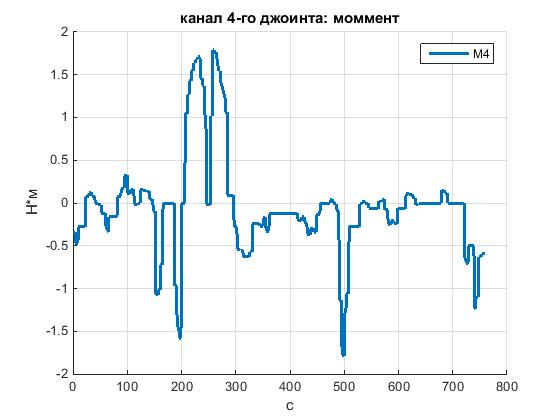
\includegraphics[width=5.5in]{./graph/m4.jpg}	
		\caption{
			\textbf{Y - канал: силы}
		}
		\label{fig_img54}
	\end{figure}
	\begin{figure}[h]
		\centering		 
		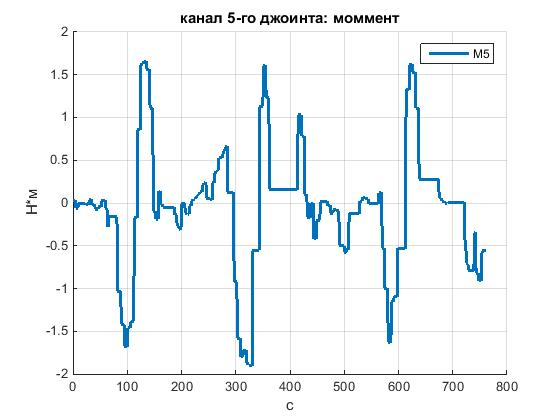
\includegraphics[width=5.5in]{./graph/m5.jpg}	
		\caption{
			\textbf{Z - канал: положения}
		}
		\label{fig_img55}
	\end{figure}
	\begin{figure}[h]
		\centering		 
		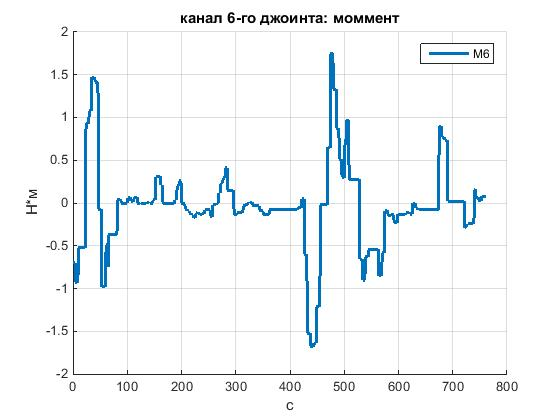
\includegraphics[width=5.5in]{./graph/m6.jpg}	
		\caption{
			\textbf{Z - канал: силы}
		}
		\label{fig_img56}
	\end{figure}
	\section{Результаты экспериментов}
	Из графиков наглядно видно, что система имеет серьёзное запаздывание, что вызвано "шаговостью" робота-манипулятора. 
	Тем не менее система корректно отрабатывает задание, следовательно, поставленная задача выполнена.
\end{document}